
\section{Finding the optimal number of robots}
To find the optimal number of robots the map tested were: the city environment map and 3 increasing size obstacle-free square maps: 5x5, 10x10, 15x15. After normalising the result parameters, the method used for establishing the optimal number of robots is evaluating the output of a weighted loss function $\mathscr{L}$ where three $\lambda$ weight are assigned to each of the result parameters. In formulas, for a generic number of robots $R$:

\begin{equation}
\mathscr{L}_R(\lambda, \ell_i)=\lambda_1 \cdot \max(\ell_i)_N + \lambda_2 \cdot \sum(\ell_i)_N + \lambda_3 \cdot \sigma(\ell_i)_N
\end{equation}

Where subscript $N$ stands for normalised, and the best configuration will be the one that satisfies the following formula:

\begin{equation}
R_{best} = \arg\min_R \mathscr{L}_R(\lambda, \ell_i)
\end{equation}
 
By acting on the parameters we can set a  lexicographical order that meets the objective we want to achieve. The $\lambda$ parameters where obtained with a simple tuning based on the fact that the most important parameter is $\lambda_1$ since it weights $max(\ell_i)$ that defines the coverage completion time, and we want to minimize it. Then on a second level we want that the total energy spent by the swarm is minimized and at last we don't want a big disparity between paths lengths since it means that are some redundant robots. The parameters of the online and offline algorithms are not the same since in the online algorithms, till the coverage is completed, each robot performs the same number of steps, so $\lambda_3$ was set to a very small value with respect to the other two parameters.
By taking advantage of the analysing performed in the previous section the simulations for this case will be run only for the Node Counting and VRP algorithms.
In the following figures all the values in the graphs will be also represented as normalised. Due to the long execution times of the Node Counting (the deterministic solution of the Greedy is almost instant), the two algorithms will be compared for maps sizes not greater than 15x15.

%%%%%%%%%%%%%%%%%%%%

\subsection{Node Counting}
A common trend in all the plots is that the maximum path length $\max (\ell_i)$ always decreases with the increasing number of robots, which is an expected intuitive result. Nevertheless there is point where increasing the number of robots is no more convenient due to the consequent increase of the total paths length $\sum (\ell_i)$. An interesting result that can be observed in the profile of the total length curve is that there are some local minima that for larger sizes of the map occur in correspondence of a higher number of robots.

%\begin{figure}[H]
\centering
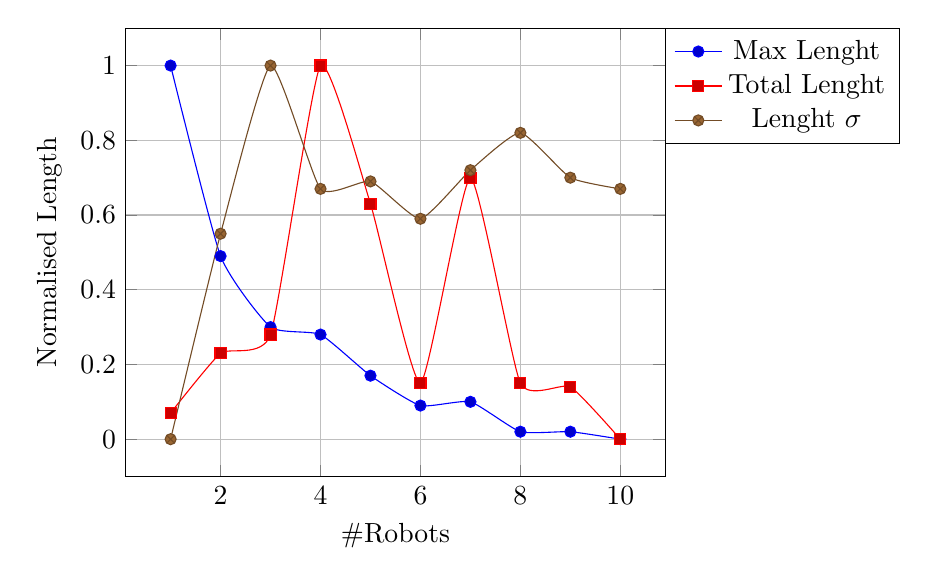
\begin{tikzpicture}
	\begin{axis}[
%		height=9cm,
%		width=9cm,
		grid=major,
                legend style = {at={(1,1)}, anchor=north west},
		xlabel=\#Robots,
		ylabel=Normalised Length,
		smooth,
		tension=0.3
	]

	\addplot coordinates {
(1, 1.00)
(2, 0.49)
(3, 0.30)
(4, 0.28)
(5, 0.17)
(6, 0.09)
(7, 0.10)
(8, 0.02)
(9, 0.02)
(10, 0.00)
	};
	\addlegendentry{Max Lenght}

	\addplot coordinates {
(1, 0.07)
(2, 0.23)
(3, 0.28)
(4, 1.00)
(5, 0.63)
(6, 0.15)
(7, 0.70)
(8, 0.15)
(9, 0.14)
(10, 0.00)
	};
	\addlegendentry{Total Lenght}

	\addplot coordinates {
(1, 0.00)
(2, 0.55)
(3, 1.00)
(4, 0.67)
(5, 0.69)
(6, 0.59)
(7, 0.72)
(8, 0.82)
(9, 0.70)
(10, 0.67)
	};
	\addlegendentry{Lenght $\sigma$}
	\end{axis}
\end{tikzpicture}
\caption{Variation of the performance indexes increasing the number of robots, for the 15x15 grid using the Node Counting algorithm}
\end{figure}


\begin{figure}[H]
\centering
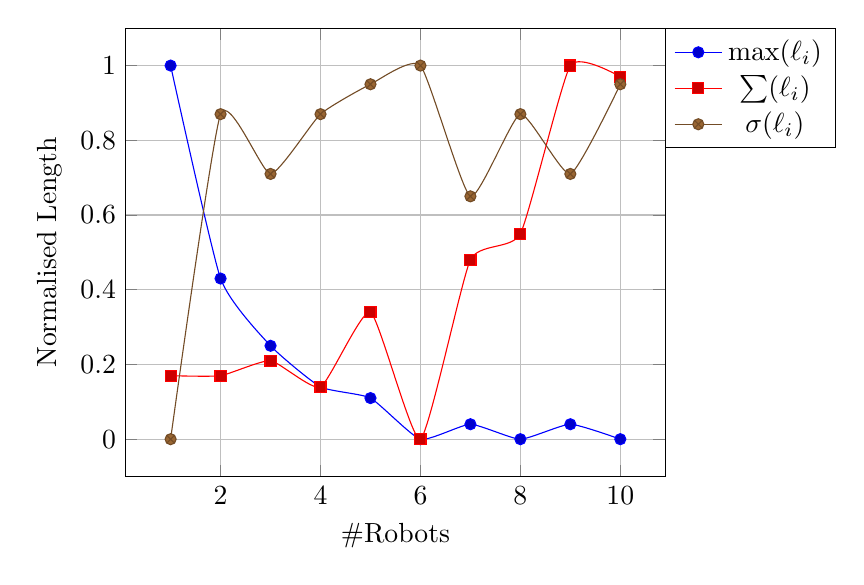
\begin{tikzpicture}
	\begin{axis}[
%		height=9cm,
%		width=9cm,
		grid=major,
                legend style = {at={(1,1)}, anchor=north west},
		xlabel=\#Robots,
		ylabel=Normalised Length,
		smooth,
		tension=0.3
	]

	\addplot coordinates {
(1, 1.00)
(2, 0.43)
(3, 0.25)
(4, 0.14)
(5, 0.11)
(6, 0.00)
(7, 0.04)
(8, 0.00)
(9, 0.04)
(10, 0.00)
	};
	\addlegendentry{$\max(\ell_i)$}

	\addplot coordinates {
(1, 0.17)
(2, 0.17)
(3, 0.21)
(4, 0.14)
(5, 0.34)
(6, 0.00)
(7, 0.48)
(8, 0.55)
(9, 1.00)
(10, 0.97)
	};
	\addlegendentry{$\sum(\ell_i)$}

	\addplot coordinates {
(1, 0.00)
(2, 0.87)
(3, 0.71)
(4, 0.87)
(5, 0.95)
(6, 1.00)
(7, 0.65)
(8, 0.87)
(9, 0.71)
(10, 0.95)
	};
	\addlegendentry{$\sigma(\ell_i)$}
	\end{axis}
\end{tikzpicture}
\caption[Perform. indexes increasing the \#robots, 5x5 grid using NC]{Performance indexes increasing the num. of robots, 5x5 grid using NC}
\end{figure}


\begin{figure}[H]
\centering
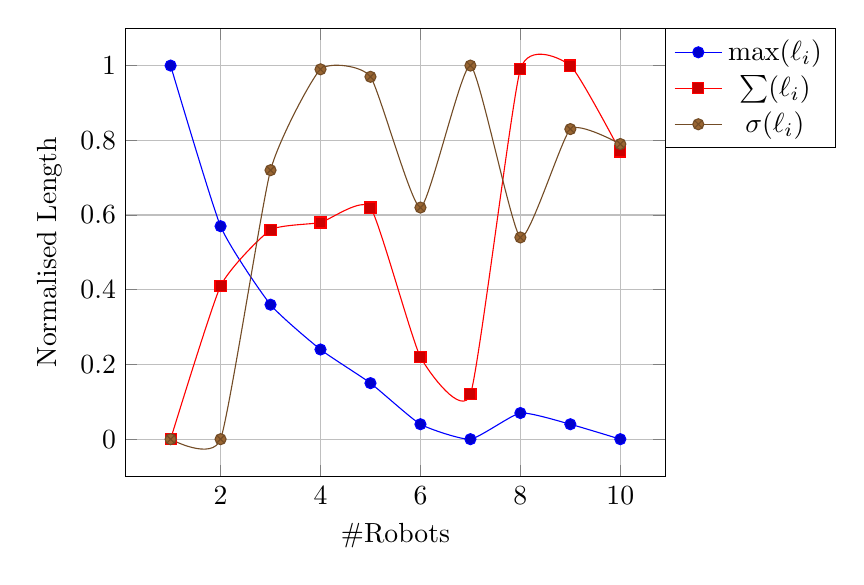
\begin{tikzpicture}
	\begin{axis}[
%		height=9cm,
%		width=9cm,
		grid=major,
                legend style = {at={(1,1)}, anchor=north west},
		xlabel=\#Robots,
		ylabel=Normalised Length,
		smooth,
		tension=0.3
	]

	\addplot coordinates {
(1, 1.00)
(2, 0.57)
(3, 0.36)
(4, 0.24)
(5, 0.15)
(6, 0.04)
(7, 0.00)
(8, 0.07)
(9, 0.04)
(10, 0.00)
	};
	\addlegendentry{$\max(\ell_i)$}

	\addplot coordinates {
(1, 0.00)
(2, 0.41)
(3, 0.56)
(4, 0.58)
(5, 0.62)
(6, 0.22)
(7, 0.12)
(8, 0.99)
(9, 1.00)
(10, 0.77)
	};
	\addlegendentry{$\sum(\ell_i)$}

	\addplot coordinates {
(1, 0.00)
(2, 0.00)
(3, 0.72)
(4, 0.99)
(5, 0.97)
(6, 0.62)
(7, 1.00)
(8, 0.54)
(9, 0.83)
(10, 0.79)
	};
	\addlegendentry{$\sigma(\ell_i)$}
	\end{axis}
\end{tikzpicture}
\caption[Perform. indexes increasing the \#robots, 10x10 grid using NC]{Performance indexes increasing the num. of robots, 10x10 grid using NC}
\end{figure}

So for the Node Counting algorithm we have that for a 5x5 map the best number of robots is 6, for the 10x10 map is 7 and for the 15x15 map is 10. The bigger leap between the last two results derives from the fact that a linear increase in the map side obviously produces a quadratic increase in the map area, thus on the size of the navigation graph. Even though no precise pattern is emerging from the relationship between number of robots and size of the map, this results give anyway an idea about the order of magnitude of the robots necessary for coverage for increasing map size.


\begin{figure}[H]
\centering
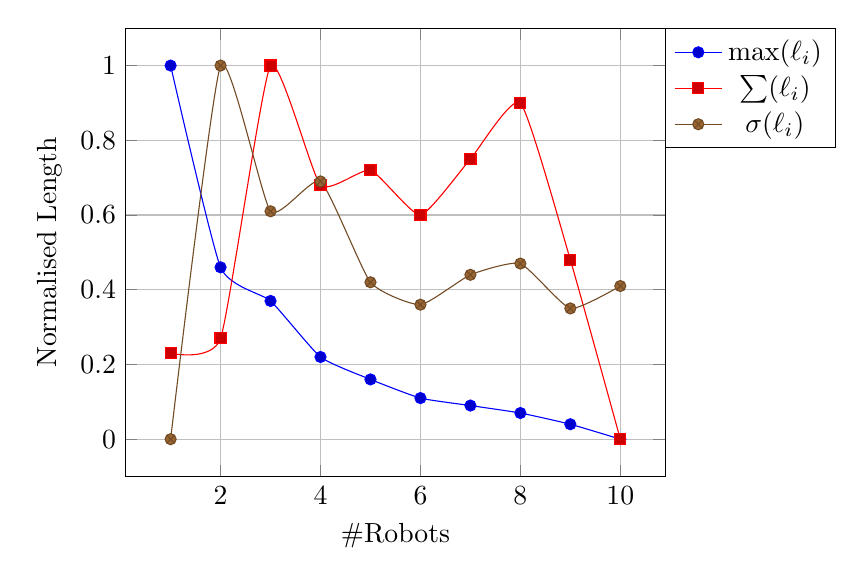
\begin{tikzpicture}
	\begin{axis}[
%		height=9cm,
%		width=9cm,
		grid=major,
                legend style = {at={(1,1)}, anchor=north west},
		xlabel=\#Robots,
		ylabel=Normalised Length,
		smooth,
		tension=0.3
	]

	\addplot coordinates {
(1, 1.00)
(2, 0.46)
(3, 0.37)
(4, 0.22)
(5, 0.16)
(6, 0.11)
(7, 0.09)
(8, 0.07)
(9, 0.04)
(10, 0.00)
	};
	\addlegendentry{$\max(\ell_i)$}

	\addplot coordinates {
(1, 0.23)
(2, 0.27)
(3, 1.00)
(4, 0.68)
(5, 0.72)
(6, 0.60)
(7, 0.75)
(8, 0.90)
(9, 0.48)
(10, 0.00)
	};
	\addlegendentry{$\sum(\ell_i)$}

	\addplot coordinates {
(1, 0.00)
(2, 1.00)
(3, 0.61)
(4, 0.69)
(5, 0.42)
(6, 0.36)
(7, 0.44)
(8, 0.47)
(9, 0.35)
(10, 0.41)

	};
	\addlegendentry{$\sigma(\ell_i)$}
	\end{axis}
\end{tikzpicture}
\caption[Perform. indexes increasing the \#robots, 15x15 grid using NC]{Performance indexes increasing the num. of robots, 15x15 grid using NC}
\end{figure}

%%%%%%%%%%%%%%%%%%%


\subsection{VRP with Floyd-Warshall}
In the following figures are plotted the results for increasing number of robots and increasing map size using the VRP Greedy coverage algorithm.

%\begin{figure}[H]
\centering
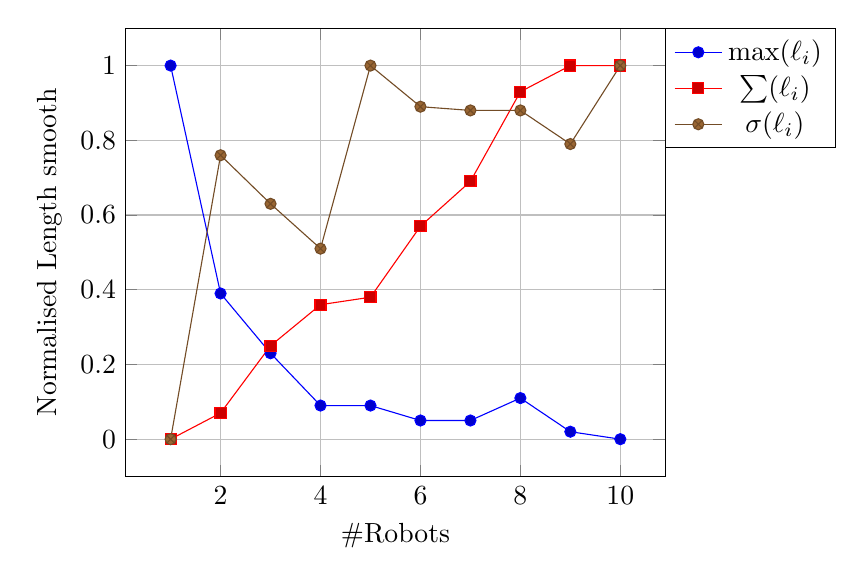
\begin{tikzpicture}
	\begin{axis}[
%		height=9cm,
%		width=9cm,
		grid=major,
                legend style = {at={(1,1)}, anchor=north west},
		xlabel=\#Robots,
		ylabel=Normalised Length
		smooth,
		tension=0.3
	]

	\addplot coordinates {
(1, 1.00)
(2, 0.39)
(3, 0.23)
(4, 0.09)
(5, 0.09)
(6, 0.05)
(7, 0.05)
(8, 0.11)
(9, 0.02)
(10, 0.00)
	};
	\addlegendentry{$\max(\ell_i)$}

	\addplot coordinates {
(1, 0.00)
(2, 0.07)
(3, 0.25)
(4, 0.36)
(5, 0.38)
(6, 0.57)
(7, 0.69)
(8, 0.93)
(9, 1.00)
(10, 1.00)
	};
	\addlegendentry{$\sum(\ell_i)$}

	\addplot coordinates {
(1, 0.00)
(2, 0.76)
(3, 0.63)
(4, 0.51)
(5, 1.00)
(6, 0.89)
(7, 0.88)
(8, 0.88)
(9, 0.79)
(10, 1.00)
	};
	\addlegendentry{$\sigma(\ell_i)$}
	\end{axis}
\end{tikzpicture}
\caption[Perform. indexes increasing the \#robots, city map using VRP]{\mbox{Performance indexes increasing the num. of robots, city map using VRP}}
\end{figure}

\begin{figure}[H]
\centering
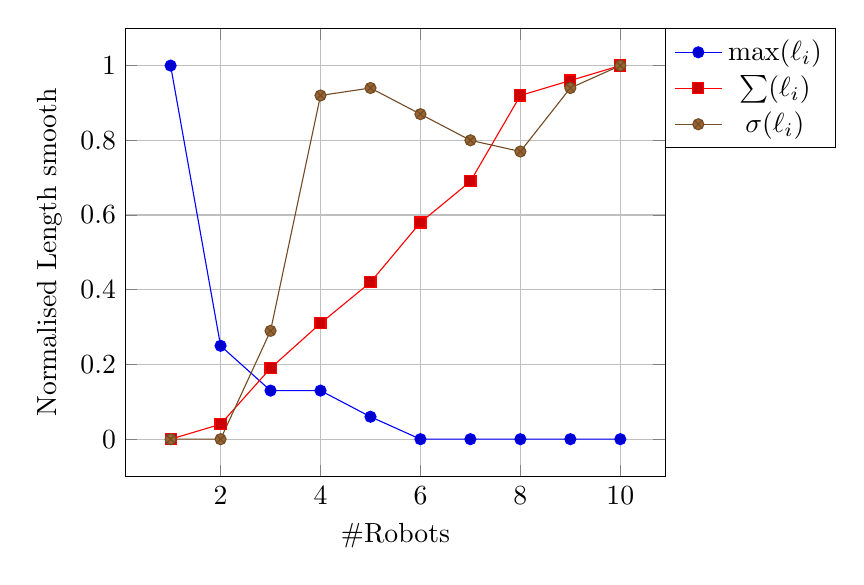
\begin{tikzpicture}
	\begin{axis}[
%		height=9cm,
%		width=9cm,
		grid=major,
                legend style = {at={(1,1)}, anchor=north west},
		xlabel=\#Robots,
		ylabel=Normalised Length
		smooth,
		tension=0.3
	]

	\addplot coordinates {
(1, 1.00)
(2, 0.25)
(3, 0.13)
(4, 0.13)
(5, 0.06)
(6, 0.00)
(7, 0.00)
(8, 0.00)
(9, 0.00)
(10, 0.00)
	};
	\addlegendentry{$\max(\ell_i)$}

	\addplot coordinates {
(1, 0.00)
(2, 0.04)
(3, 0.19)
(4, 0.31)
(5, 0.42)
(6, 0.58)
(7, 0.69)
(8, 0.92)
(9, 0.96)
(10, 1.00)
	};
	\addlegendentry{$\sum(\ell_i)$}

	\addplot coordinates {
(1, 0.00)
(2, 0.00)
(3, 0.29)
(4, 0.92)
(5, 0.94)
(6, 0.87)
(7, 0.80)
(8, 0.77)
(9, 0.94)
(10, 1.00)
	};
	\addlegendentry{$\sigma(\ell_i)$}
	\end{axis}
\end{tikzpicture}
\caption[Perform. indexes increasing the \#robots, 5x5 grid using VRP]{Performance indexes increasing the num. of robots, 5x5 grid using VRP}
\end{figure}

For the VRP algorithm we find that for a 5x5 map the best number of robots is 2, for the 10x10 map is 3 and for the 15x15 map is 5. We can clearly see how using this kind of algorithm the best number of robots is on average less than the one needed for Node Counting, that is a desirable property in term of resource saving.

\input{tex/graphs/VRP_FW_10x10_normalised}

\begin{figure}[H]
\centering
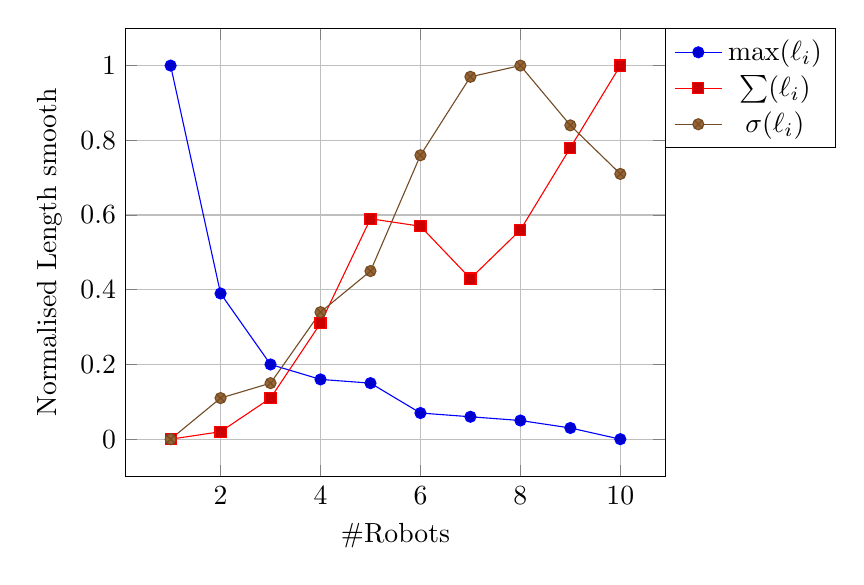
\begin{tikzpicture}
	\begin{axis}[
%		height=9cm,
%		width=9cm,
		grid=major,
                legend style = {at={(1,1)}, anchor=north west},
		xlabel=\#Robots,
		ylabel=Normalised Length
		smooth,
		tension=0.3
	]

	\addplot coordinates {
(1, 1.00)
(2, 0.39)
(3, 0.20)
(4, 0.16)
(5, 0.15)
(6, 0.07)
(7, 0.06)
(8, 0.05)
(9, 0.03)
(10, 0.00)
	};
	\addlegendentry{$\max(\ell_i)$}

	\addplot coordinates {
(1, 0.00)
(2, 0.02)
(3, 0.11)
(4, 0.31)
(5, 0.59)
(6, 0.57)
(7, 0.43)
(8, 0.56)
(9, 0.78)
(10, 1.00)
	};
	\addlegendentry{$\sum(\ell_i)$}

	\addplot coordinates {
(1, 0.00)
(2, 0.11)
(3, 0.15)
(4, 0.34)
(5, 0.45)
(6, 0.76)
(7, 0.97)
(8, 1.00)
(9, 0.84)
(10, 0.71)
	};
	\addlegendentry{$\sigma(\ell_i)$}
	\end{axis}
\end{tikzpicture}
\caption[Perform. indexes increasing the \#robots, 15x15 grid using VRP]{\mbox{Performance indexes increasing the num. of robots, 15x15 grid using NC}}
\end{figure}

In figure \ref{fig:VRPFW_execTime} is presented a comparison plot for the algorithm execution time with an increasing size of the maps.  The longest execution time has been recorded for the computation of the path for one robot in a 40 by 40 free map, for a value of $7\e{2}$ seconds, roughly 12 minutes.


\begin{figure}[H]
\centering
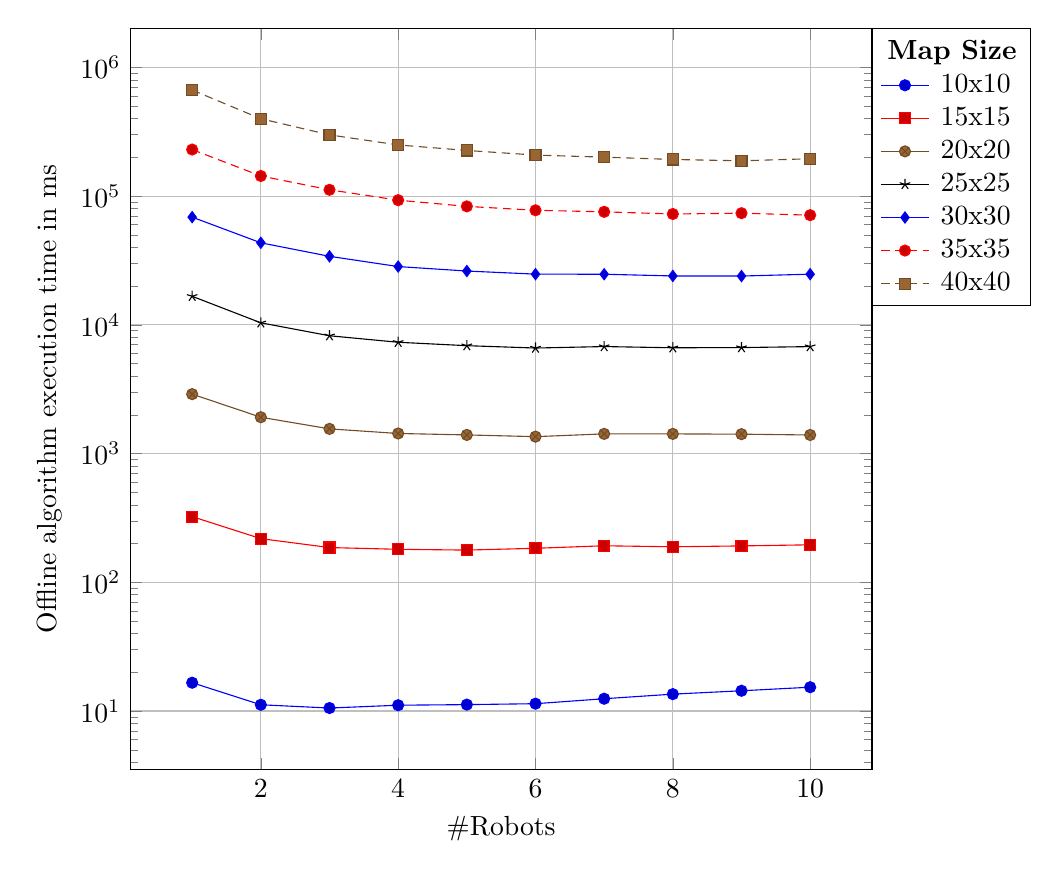
\begin{tikzpicture}
	\begin{semilogyaxis}[
		height=11cm,
		width=11cm,
                legend style = {at={(1,1)}, anchor=north west},
		grid=major,
		xlabel=\#Robots,
                   ylabel=Offline algorithm execution time in ms
	]

        \addlegendimage{empty legend}
        \addlegendentry{\hspace{-.6cm}\textbf{Map Size}}

%	\addplot coordinates {
%		(1, 0.962165)
%		(2, 0.999812)
%		(3, 3.32455)
%		(4, 1.33711)
%		(5, 1.26769)
%		(6, 4.00359)
%		(7, 4.45941)
%		(8, 1.33102)
%		(9, 1.38427)
%                (10, 3.06631)
%	};
%	\addlegendentry{5x5}

	\addplot coordinates {
		(1, 99.5812/6)
		(2, 67.1215/6)
		(3, 63.3223/6)
		(4, 66.5972/6)
		(5, 67.303/6)
		(6, 68.4257/6)
		(7, 74.7808/6)
		(8, 81.1845/6)
		(9, 86.226/6)
                (10, 91.9106/6)
	};
	\addlegendentry{10x10}

	\addplot coordinates {
		(1, 1941.57/6)
		(2, 1310.12/6)
		(3, 1117.07/6)
		(4, 1082.52/6)
		(5, 1067.53/6)
		(6, 1102.4/6)
		(7, 1153.16/6)
		(8, 1132.38/6)
		(9, 1150.22/6)
                (10, 1173.2/6)
	};
	\addlegendentry{15x15}

	\addplot coordinates {
		(1, 17361.1/6)
		(2, 11490/6)
		(3, 9328.54/6)
		(4, 8591.75/6)
		(5, 8372.56/6)
		(6, 8116.5/6)
		(7, 8529.95/6)
		(8, 8526.77/6)
		(9, 8485.28/6)
                (10, 8361.64/6)
	};
	\addlegendentry{20x20}

	\addplot coordinates {
		(1, 99929.9/6)
		(2, 62180.2/6)
		(3, 49326.2/6)
		(4, 43910.5/6)
		(5, 41311.1/6)
		(6, 39607.3/6)
		(7, 40667/6)
		(8, 39792/6)
		(9, 39942.7/6)
                (10,40629.5/6)
	};
	\addlegendentry{25x25}

	\addplot coordinates {
		(1, 411589/6)
		(2, 260044/6)
		(3, 204265/6)
		(4, 170023/6)
		(5, 156969/6)
		(6, 148516/6)
		(7, 148225/6)
		(8, 143764/6)
		(9, 143510/6)
                (10, 148387/6)
	};
	\addlegendentry{30x30}

	\addplot coordinates {
		(1, 1.37889e+06/6)
		(2, 859312/6)
		(3, 671124/6)
		(4, 557420/6)
		(5, 498969/6)
		(6, 465257/6)
		(7, 452598/6)
		(8, 435339/6)
		(9, 441815/6)
                (10, 426400/6)
	};
	\addlegendentry{35x35}

	\addplot coordinates {
		(1, 3.99748e+06/6)
		(2, 2.39203e+06/6)
		(3, 1.79249e+06/6)
		(4, 1.49702e+06/6)
		(5, 1.35637e+06/6)
		(6, 1.24861e+06/6)
		(7, 1.20327e+06/6)
		(8, 1.15456e+06/6)
		(9, 1.12716e+06/6)
                (10, 1.16961e+06/6)
	};
	\addlegendentry{40x40}
	
	\end{semilogyaxis}
\end{tikzpicture}
\caption{VRP-FloydWarshall:  Different execution times for growing map sizes}
\label{fig:VRPFW_execTime}
\end{figure}






